\chapter{Computer Science Background}
\label{ch:computerscience}

A graph, or network, is a collection of nodes which are connected by edges.
A graph is denoted as $G=(V,E)$ in which $v \in V$ is a vertex, or node, and $e \in E$ is an edge~\cite{cai_comprehensive_2017}.
If a graph has multiple types of nodes and/or edges, it is called heterogeneous.
Alternatively, a graph that has only one type of node and one type of edge is called homogeneous~\cite{cai_comprehensive_2017}.

Analysis of networks is used in many different fields to understand the community structure of the network and the relationships between entities~\cite{cai_comprehensive_2017}.
It also helps gain insight on the hidden information and patterns in the network~\cite{cai_comprehensive_2017}.
Network analysis have been used in many applications such as relationship prediction, entity classification, clustering, and visualization~\cite{goyal_graph_2018}.

\ac{NRL} is a machine learning approach that learns embeddings for nodes of a network in a latent, low-dimensional vector space, without compromising node content, network topology, and other information~\cite{zhang_network_2017}.
The topological and structural properties of a node are encoded into its embedding, and the distance between nodes in the vector space captures the relationships between them.
Since each node is represented by a vector that contains its information of interest, computing mapping functions or distance matrices on the embedding can help avoid high complexity during network analysis.
Thus, \ac{NRL} methods have two main goals: to be able to reconstruct the original network from the learned embedding and to be able to use the learned embedding space to effectively support network interface~\cite{sheikh_gat2vec:_2018}.

\section{Background on Network Biology}

Relationships in systems biology are often represented as networks, which allows analysis and modeling of the data using computational methods.
With the emergence of the field of systems biology, many biological networks have been created and analyzed such as protein-protein interactions, gene regulatory networks, and metabolic networks.
The study of such networks help in the understanding of human disease, mechanisms of action of drugs, and complex biological systems~\cite{dancik_properties_2013}.

\subsection{Biological Network Topology}

The structure of a network plays an important role in analyzing and understanding its performance.
The most common topological features (e.g., degree distribution, distance, clustering coefficient) are discussed below.

The degree of a node is the number of relations it has, a node with high degree has a better connection in the network, therefore it plays a more important role in preserving the network structure.
Biological networks usually consist of a small number of nodes that are highly connected (hubs), and a large number of nodes that have fewer connections, which is known as “scale-free” format~\cite{zhu_getting_2007}.
This network format follows a power-law distribution $k^{-a}$ where k is the degree of a fraction of nodes and $a>1$~\cite{broido_scale-free_2019}.

The geodesic distance between two nodes is defined as the length of the shortest path between them.
On the other hand, the diameter of a network is the maximum shortest path length between all pairs of nodes.
The approximate distance between nodes in a network can be measured by calculating the average distance and diameter.
A network with small diameter means that on average two nodes are connected by relatively short paths.
This type of graph is generally known as a “small world” network~\cite{zhu_getting_2007}.

The clustering coefficient of a node is the percentage of existing relations among its neighborhood.
It can be calculated by the number of edges between nodes in the neighborhood divided by the total number of edges that are possible between them, which gives a value between 0 and 1.
A “small world” network usually has a high clustering coefficient, which indicates that nodes in the network tend to form groups~\cite{zhu_getting_2007}.
On the other hand, a network that was created randomly has a low clustering coefficient, usually very close to 0 $(C \approx 0)$~\cite{newman_random_2002}.

\section{Random Walk Representation Learning Methods}

A random walk is a stochastic process in which a path is created by iteratively randomly choosing a neighbor of the last node in the walk.
Random walks are useful for detecting communities and capturing community information~\cite{perozzi_deepwalk:_2014}.
For the purpose of \ac{NRL}, a stream of short random walks is used to extract the network information, and several walkers can be used to explore different parts of the same graph at the same time~\cite{perozzi_deepwalk:_2014}.

\subsection{Language Models}

Language models are an important part of natural language processing, which is a branch of artificial intelligence that aims to enable computers to interact, analyze, and process natural language.
The objective of a language model is to assign probabilities specific sequence of words appearing in a corpus.
For a sentence with finite sequence of words from a given vocabulary, the goal is to maximize the probability of a word over all the training corpus~\cite{perozzi_deepwalk:_2014}.
To use a language model on short random walks created from a graph, one can generalize the model by processing the random walks as a special language with nodes as words~\cite{perozzi_deepwalk:_2014}.

\subsection{SkipGram and GloVe}

SkipGram is a language model that attempts to predict the context of a word by maximizing the probability of co-occurrence among the words that appear within a window in a sentence~\cite{perozzi_deepwalk:_2014}.
This can be done by training a neural network with pairs of words within a certain window from the training corpus, the probability of the co-occurrence is then calculated by the number of times each pair appeared in the training~\cite{mccormick_word2vec_nodate}.
However, since the goal is to learn latent representations rather than the probability of node co-occurrences, a mapping function is introduced to the probability calculation~\cite{perozzi_deepwalk:_2014}.

\ac{GloVe} is another language model that uses a count matrix factorization approach.
It learns word representations by calculating their ratio of the co-occurrence probability instead of raw co-occurrence probability, which is said to encode meaningful global information~\cite{pennington_glove:_2014}.

\subsection{DeepWalk}


DeepWalk is an unsupervised scalable representation learning model that learns latent representations by obtaining information from short random walks.
The algorithm of the model consists of two main steps:
\begin{enumerate}[1.]
    \item Perform random walks on the nodes in the graph and generate short sequences of nodes
    \item Run SkipGram using the paths generated in the first step to learn features of nodes and create node embeddings.
\end{enumerate}
The model also uses hierarchical softmax to approximate the probability distribution, since using softmax as an activation function would be computationally expensive, with a computation time of $O(|V|)$.
In hierarchical softmax, a binary tree, with the nodes of the graph as leaves, is used to handle the computation problem by factorizing the conditional probability.
The probability of a given node $v_{i}$ is computed by calculating the probability of each sub-path from the root node to the node $v_{i}$, which reduces the computation time to $O(log|V|)$~\cite{perozzi_deepwalk:_2014}.
\begin{figure}[!ht]
    \center{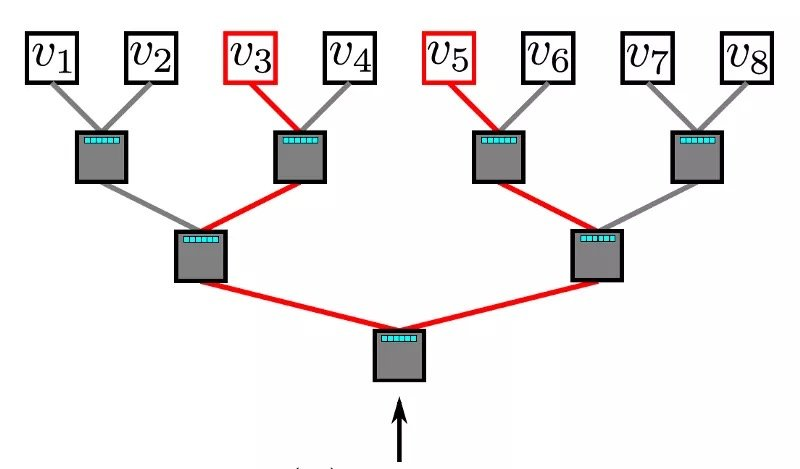
\includegraphics[scale=0.4]
    {figures/hs.jpg}
    \captionsetup{justification=centering}
    \caption[A schematic diagram of the hierarchical Softmax]{\label{fig:hs} A schematic diagram of the hierarchical Softmax. Image adapted from~\cite{perozzi_deepwalk:_2014}}
    }
\end{figure}


\subsection{Node2vec}\label{subsection:node2vec}

\begin{figure}[ht!]
    \center{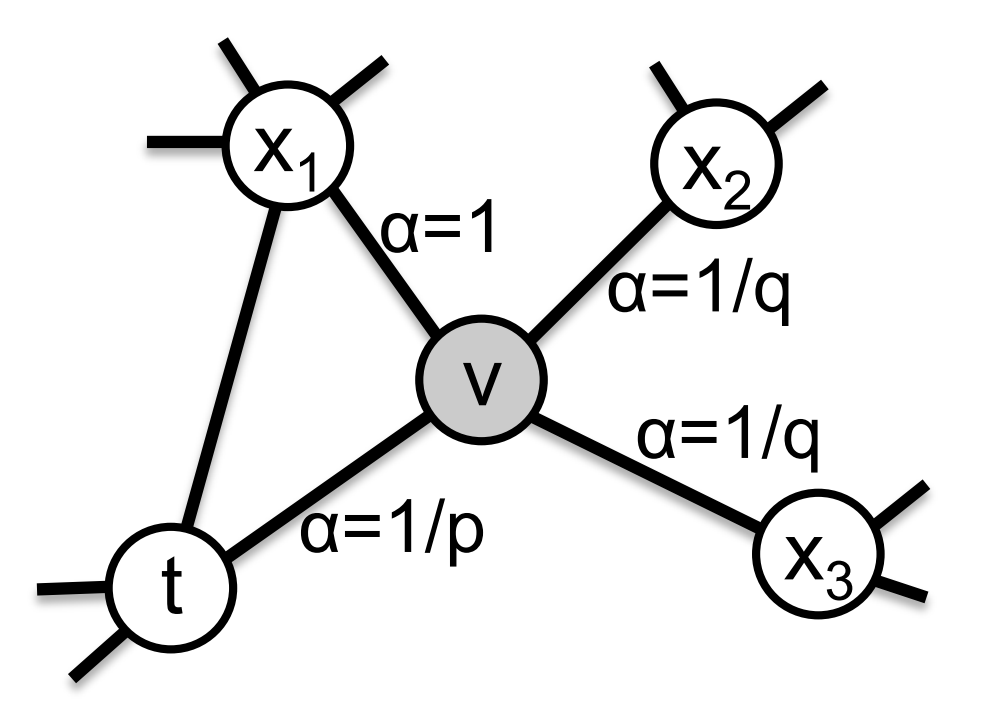
\includegraphics[scale=0.25]
    {figures/node2vec.png}
    \captionsetup{justification=centering}
    \caption[An illustration of node2vec transition calculations]{\label{fig:node2vec}  Random walk evaluation for next step transition for $v$. Edge labels indicate the search bias. Image adapted from~\cite{grover_node2vec:_2016}}
    }
\end{figure}

Node2vec is a semi-supervised approach that learns scalable latent features in networks.
This model is very similar to DeepWalk with two additional parameters: $p$ and $q$.
The return parameter, $p$, controls the probability of revisiting nodes in a walk.
A high value of $p$ means that it is less likely to revisit a node for the next two steps.
If $p$ is low, it is more likely to revisit the node immediately.
Having a low $p$ parameter ensures that the walk stays local.
The $q$ parameter deals with “inward” and “outward” nodes.
If $q$ > 1, the random walk is more likely to visit a node that is close to the previous node, which means that it focuses more on the local structures.
If $q$ < 1, then the walk is biased toward nodes that are further away from the previous node, which encourages exploration of the graph~\cite{grover_node2vec:_2016}.

\section{Other Representation Learning Methods}

\subsection{Translational Distance Models}

The idea of translational distance methods is to calculate the possibility of a fact by measuring the distance between two entities using distance-based scoring functions~\cite{wang_knowledge_2017}.
Translational models have multiple applications in biomedical literature, including drug-drug interaction prediction from drug knowledge graph~\cite{abdelaziz_large-scale_2017, wang_predicting_2017} and disease prediction and clustering from symptom-disease network~\cite{zhao_contextcare:_2017}.

\subsubsection{TransE}

TransE is an energy-based model that represents relationships as translations in the embedding space.
Assuming there is a directed graph with entities and edges in the form of (head, relation, tail), or $(h, r, t)$, which indicated that there is a relationship between the head and tail entities.
Then the embedding of the two entities \textit{h} and \textit{t} should be close to one another plus a translation vector \textit{r}, i.e., $h + r \approx t$ when $(h, r, t)$ holds.
This approach learns only one embedding for each entity and each relationship, i.e., 1-to-1 relationships~\cite{bordes_translating_2013}.

\subsubsection{TransH}
TransH, or translation on hyperplane, tries to solve the problem in dealing with 1-to-N/N-to-N/N-to-1 relations in TransE by interpreting the translation vector on a hyperplane so that an entity will have distributed representations when involved in different relations.
For $(h, r, t)$, the relation \textit{r} will have a translation vector $d_{r}$ which will be projected in the relation-specific hyperplane $w_{r}$, the embedding \textit{h} and \textit{t} are projected into the hyperplane as \textit{h’} and \textit{t’}, respectively, which are expected to be connected by a translation vector $d_{r}$ on the hyperplane~\cite{wang_knowledge_2014}.

\subsubsection{TransR}

While both TransE and TranH assume that the embeddings of entities and relations are in the same space, TransR suggests creating entities and relations in different spaces and performs the translation depending on the relation space.
A a projection matrix $M_{r}$ is generated for each relation \textit{r}, which projects entities from the entity space to relation space.
For a triple $(h, r, t)$, $h$ and $t$ entity embeddings are projected into \textit{r}-relation space with operation $M_{r}$~\cite{lin_learning_2015}.
Though TransR has improved compared to the previous translational models, it has a few limitations that can affect its performance.
For example, even though entities linked by relations can have various types and attributes, it maps all relations to the same mapping matrix $M_{r}$.
Also, mapping matrices are determined by the relations alone, despite the fact that there is an interactive process between an entity and a relation~\cite{ji_knowledge_2015}.

\subsection{Matrix Factorization Methods}

As the name suggests, these algorithms factorize a matrix which is formed from connections between nodes to obtain embeddings.
The matrix representing the connections can be created using different data like the adjacency matrix, the Laplacian, or the node transition probability matrix~\cite{goyal_graph_2018}.
Matrix factorization methods have been utilized before for drug-target interaction prediction using similarity profiles~\cite{ezzat_drug-target_2017, yamanishi_dinies:_2014} and in gene-disease networks using gene similarity and disease similarity matrices~\cite{zeng_probability-based_2017}.
One important advantage of these methods is that they can preserve the global structure of a network by considering global nodes proximity.
However, they are unscalable to large graphs because they are time and space consuming~\cite{cai_comprehensive_2017}.

\subsubsection{HOPE}

\ac{HOPE} is a graph embedding approach that attempts to preserve the asymmetric transitivity in the graph, which is important in capturing its structure.
Asymmetric transitivity represents the correlation between directed edges, which is that if there is a directed edge from $u$ to $v$, then there is probably a directed edge from $v$ to $u$.
In \ac{HOPE}, an adjacency matrix is used to derive two polynomial matrices, which are then used to generate generalized singular values for each polynomial matrix and their corresponding singular vectors.
The two generalized singular values vectors can be combined and then used along with the singular vectors to create the optimal embeddings~\cite{ou_asymmetric_2016}.

\subsubsection{GraRep}

\ac{GraRep} is an approach that captures the graph’s global structure information using an extended version of SkipGram~\cite{cao_grarep:_2015}.
\ac{GraRep} learns the different $k$-step relation information with different $k$ values among nodes form the graph by utilizing different global transition matrices defined over the graph.
In this model, nodes with common $k$-step neighbors should have similar latent features~\cite{cao_grarep:_2015}.
The method starts by creating three matrices, an adjacency matrix $S$, which indicates the presence or absence of edges between given node pair, degree matrix $D$, which contains information about the number of connections each node has, and 1-step probability transition matrix $A$ which indicates the probability of transition between node pair within one step.
\begin{equation}
    \label{eq:grarep_01}
    A = D^{-1}S
\end{equation}
$k$-step transition probability matrix for each $k$-step can be computed.
Where $A^{k}_{i,j}$ refers to the transition probability between $v_{i}$ and $v_{j}$ in which the transition contains exactly $k$-step(s).
For each $k$-step, the positive log probability matrix is produced and representations are generated separately, then all $k$-step representations are concatenated together to form the final representation.

\subsection{Deep Learning Methods}

While the previously described methods perform poorly on large and real world information networks and face challenges in handling non-linear data structures~\cite{cui_survey_2017}, deep learning methods solve these issues by incorporating autoencoders, which contain multiple nonlinear functions, and deep neural networks, which are robust and effective because of their multi-layered architecture~\cite{cai_comprehensive_2017}.
These kind of models have been used in tasks like utilizing electronic health records for risk prediction~\cite{cheng_risk_2016}, and predicting polypharmacological side effects~\cite{zitnik_modeling_2018}.

\subsubsection{LINE}

\ac{LINE} is a model proposed to handle the issue of embedding large information networks into low dimensional vector space.
\ac{LINE} optimizes an objective functions that can preserve both the local (i.e.,~first-order proximity) and global (i.e.,~second-order proximity) structures of multiple types of networks (e.g.~directed, undirected, and/or weighted)~\cite{tang_line:_2015}.

First-order proximity, which is the local pairwise proximity between nodes in the network, for an undirected edge$(i,j)$ can be found by defining the joint probability between two nodes as shown in equation~\ref{eq:line_01}.
Where $u_{i}$ is the low-dimensional representation (vector) of the node $v_{i}$.
The objective function is optimized by minimizing the difference between two probability distributions.
First-order proximity can only be applied to undirected edges in this model~\cite{tang_line:_2015}.
\begin{equation}
    \label{eq:line_01}
    p_{1}(v_{i}, v_{j}) = \frac{1}{1+ \exp{(-u_{i}^T .u_{j})}}
\end{equation}

Second-order proximity assumes that nodes with many connections to other nodes are similar to each other.
Also, each node is perceived as a "context" and nodes that have similar distributions over the "contexts" are presumed to be similar.
For each edge$(i,j)$, the conditional distribution of "context" $v_{i}$ is defined in equation~\ref{eq:line_02} where $u_{i}$ is the representation of the node $v_{i}$ itself while $u_{i}^{'}$ is the representation of the node as "context" to other nodes and $|V|$ is the number of nodes or "contexts".
Similar to first-order proximity, the objective function of the second-order proximity is calculated by minimizing the difference between two probability distributions~\cite{tang_line:_2015}.

\begin{equation}
    \label{eq:line_02}
    p_{2}(v_{i}| v_{j}) = \frac{\exp(u_{j}^{'T} .u_{i})}{\sum_{k=1}^{|V|} \exp{(u_{k}^{'T} .u_{i})}}
\end{equation}

The model can preserve both the first-order and second-order proximity by concatenating the embedding trained by both methods for each node~\cite{tang_line:_2015}.

\subsubsection{SDNE}\label{subsection:SDNE}

\ac{SDNE} model aims to capture the highly non-linear structure of networks and preserve their local and global structures.
\ac{SDNE} is a semi-supervised autoencoder model that contains multiple layers of nonlinear mapping functions to capture the nonlinear network.
Then, the first-order proximity is used by the supervised component to capture the local structure while the second-order proximity is used by the unsupervised component to preserve the global structure of the network~\cite{wang_structural_2016}.

The neighborhood for each node is reconstructed to preserve the second-order proximity, and the pairwise similarities for a small portion of node pairs are obtained to preserve the first-order proximity, this creates an adjacency matrix which is the input to the autoencoder.
The model also introduces a penalty on the reconstruction error for non-zero elements because while the presence of links indicate similarity between nodes, the absence of links does not necessarily mean dissimilarity.
Parameter $\alpha$ balances the weight between first-order and second-order proximity, when $\alpha=0$, the model performance is dependent on second-order proximity, as $\alpha$ gets larger, the model focuses on first-order proximity.
The $\beta$ parameter controls the reconstruction weight of the non-zero elements in training set.
The larger $\beta$ is, the more susceptible the model is to reconstructing non-zero elements~\cite{wang_structural_2016}.

\section{Application of Network Representation Learning}

\ac{NRL} methods have been used in several tasks including node classification, node ranking, node clustering and edge prediction.

In node classification, the \ac{NRL} model learns latent features from labelled nodes, then assigns a class label for each node in the graph based on those features.
Thus, similar nodes will have similar labels~\cite{cui_survey_2017}.
Node classification can be used for classifying proteins according to their biological functions~\cite{grover_node2vec:_2016}.

The aim behind node ranking is to rank top $k$ nodes of interest to a given node based on criteria like similarity.
One example of an approach using such task is GuiltyTargets~\cite{muslu_guiltytargets:_2019}, which is a recently developed model that uses gat2vec~\cite{sheikh_gat2vec:_2018}, an \ac{NRL} approach extending DeepWalk, to map a protein-protein interaction network that is annotated with differential gene expression, then using machine learning methods a ranking is assigned for candidate drug targets~\cite{muslu_guiltytargets:_2019}.

The aim of node clustering is to group similar entities together.
General clustering methods like k-cluster or k-nearest neighbours are applied on the node embeddings to create clusters.
This task is particularly useful for discovering related drugs or proteins~\cite{hamilton_representation_nodate}.

The edge prediction, or link prediction, task aims to predict missing edges between nodes in a graph using the learned features.
This is possible because even though the representation is low-dimensional, it preserves the structure of the graph, so these embeddings are rich with information and can be used for edge prediction.
This is one of the most common tasks used in biological network analysis because biological networks are never complete and thus new edges can always be discovered~\cite{hamilton_representation_nodate}.
